\chapter{Aufstellen der Bewertungskriterien für die Analyse} \label{Bewertungskriterien}

Für die Evaluierung der Frameworks wird zunächst ein Katalog mit Bewertungskriterien angefertigt, anhand dessen die einzelnen Frameworks bewertet werden. Der Katalog besteht dabei aus Kriterien, die alle in Kapitel \ref{Anforderungsanalyse} vorgestellten Anforderungen an die Frameworks überprüfen sollen. Zusätzlich werden noch Kriterien aufgenommen, die durch eine Umfrage ermittelt wurden. 
\\
\\
Oben erwähnte Umfrage richtete sich an (ehemalige) Studierende der Fachhochschule Dortmund, welche angaben, bereits Erfahrungen in der mobilen Anwendungsentwicklung gesammelt zu haben. Die Fragestellung der Umfrage lautete: „Welche Kriterien halten Sie für wichtig in der Entwicklung mit Frameworks für hybride, bzw. Cross-Platform-Anwendungen?“ (E-Mail siehe Anhang) Die Befragten antworteten hierauf mit einem Freitext, indem sie die für sich wichtigen Kriterien zur Bewertung von Frameworks aufzeigten. Diese Kriterien wurden in einem Dokument (siehe CD-ROM im Anhang) gesammelt und Mehrfachnennungen entsprechend gekennzeichnet. Ein Kriterium, welches von mehreren Befragten als wichtig beschrieben wurde, bekommt bei der Evaluation eine höhere Gewichtung zugeschrieben, als ein Kriterium, welches nur von einem Befragten genannt wurde. Aus dieser Zusammenfassung der ermittelten Bewertungskriterien wurde anschließend eine Matrix (siehe Abbildung \ref{fig:Bewertungskriterien_1}-\ref{fig:Bewertungskriterien_3}) erstellt. Der Grad der Erfüllung eines Kriteriums wird an der Anzahl an Punkten zu erkennen sein, die vergeben werden. Hier ist eine Skala von 1 bis 5 (gar nicht bis voll erfüllt) vorgesehen. Wobei hier zu jedem Kriterium zunächst definiert werden muss, was „voll erfüllt“ bedeutet. Neben diesen Kriterien wird es auch Kriterien geben, welche nur mit „vorhanden“ und „nicht vorhanden“ bewertet werden können.

\section{Kategorie Kosten und Lizenz} 

In der Kategorie Kosten und Lizenz gibt es einen Sonderfall bei dem Punkt „Lizenzmodell“. Es ist hier nicht möglich eine konkrete Abstufung von „gut“ nach „schlecht“ in 5 Kategorien zu schaffen, da verschiedene Lizenzmodelle verschiedene Vor- und Nachteile aufweisen können. So wird sich darauf beschränkt, lediglich eine kurze Beschreibung des jeweiligen Lizenzmodells, sofern es eins gibt, zu formulieren. 
\\
\\
Die Punkte „Fixkosten“, „Lizenzkosten“ und „Supportkosten“ werden in 5 Abstufungen von „gratis“ bis „teuer“ unterteilt. Die exakten Geldwerte für die Grenzen der Abstufungen werden sich aus dem günstigsten und teuersten Preis, welche sich zu den Frameworks ermitteln lassen, ergeben.

\section{Kategorie Support und Community}

Bezüglich des Punktes 2)a) „Support/Wartung vom Hersteller“ (siehe Abbildung \ref{fig:Bewertungskriterien_1}) wird der Umfang des Supports pro Framework ermittelt und anhand dessen die Abstufung vorgenommen. Dies umfasst zum Beispiel telefonischen Support, ein Ticket-System oder ein moderiertes Forum. Die Qualität von Punkt 2)b) „Dokumentation“ wird unter anderem am Umfang der Dokumentation selber und am Update-Zyklus bemessen, d.h. wie schnell wird die Dokumentation entsprechend Änderungen am Framework aktualisiert? Bei der Untersuchung der Größe der Community werden, falls vorhanden, das Framework eigene Forum und weitere Entwicklerforen nach Anzahl Threads mit Themen, die sich auf das jeweilige Framework beziehen, durchleuchtet. Das Schulungsangebot wird sowohl nach Qualität als auch nach Quantität beurteilt: Das bedeutet, dass unterschieden wird, ob nur Online- oder auch Anwesenheitsschulungen angeboten werden. Hierbei spielt es auch eine Rolle an wie vielen unterschiedlichen Standorten und wie häufig Schulungen angeboten werden. Zudem wird der Angebotsumfang an Schulungen hinsichtlich einer Aufteilung von Anfänger- bis Spezialschulungen bewertet.

\section{Kategorie Entwicklung}

In der Kategorie „Entwicklung“ (siehe Abbildung \ref{fig:Bewertungskriterien_1}) werden für die Leichtigkeit der Installation und Benutzung des Frameworks Punkte von 1 bis 5 vergeben: 1 bedeutet kompliziert und aufwändig und 5 bedeutet automatisiert und intuitiv. Als „Einarbeitungszeit“ wird in diesem Falle die Zeit von der Fertigstellung der Installation bis nach dem Schreiben der ersten funktionierenden Seite der Anwendung angesehen. Hier gilt je kürzer, desto besser. Bei Punkt 3)c) „plattformübergreifend nutzbarer Code“ inwieweit der mit dem jeweiligen Framework erzeugte Code plattformübergreifend nutzbar ist, beziehungsweise wie hoch der Anteil des plattformspezifischen Codes ist. Hier gilt entsprechend, je mehr Code plattformübergreifend nutzbar ist, desto besser. Unter „Umfang Bibliotheken/Templates“ wird verstanden, wie viele Bausteine mit dem Framework sozusagen mitgeliefert werden, die einzelne Funktionalitäten kapseln und einfach in den Code zu integrieren sind.

\section{Kategorie Hersteller}

Die „Bekanntheit/Größe des Herstellerunternehmens“ des jeweiligen Frameworks wird anhand der Unternehmensgröße, des Bekanntheitsgrads, der Produktpalette und Einsätze der Produkte gewertet. Bei dem Punkt „Entwicklungsstadium des Frameworks“ (siehe Abbildung \ref{fig:Bewertungskriterien_1}) wird in die Wertung mit einbezogen, ob sich das Framework noch in einer Beta-Version befindet, oder es schon ein Release gibt. Zudem wird betrachtet, wie viele Updates und Bugfixes bereits vorgenommen wurden und wie viel von dem was das Framework laut Hersteller leisten soll bereits umgesetzt oder noch in Planung ist. Eine „Ja“-„Nein“-Unterscheidung gibt es bei dem Punkt „Weiterentwicklung des Frameworks“. Hierbei ist positiv zu bewerten, wenn das Framework nachweislich noch weiterentwickelt werden soll, um mit den Änderungen und der Weiterentwicklung der einzelnen Plattformen mithalten zu können.

\section{Kategorie OS-Versionen}

„Reaktionszeit auf OS-Update“ (siehe Abbildung \ref{fig:Bewertungskriterien_1}) beschreibt die Zeit, die benötigt wurde um nach einem Update eines Betriebssystems, wie zum Beispiel Android, das Framework entsprechend anzupassen oder zu erweitern. Mit dem Punkt „Abwärts-kompatibilität“ wird bewertet, bis zu welcher OS-Version das Framework anwendbar ist. Hier ist zum Beispiel für Android nicht ohne Bedeutung, dass weiterhin Version 4.x unterstützt wird, die unter den Android Versionen immer noch einen großen Marktanteil annehmen\footcite{AndroidMarktanteil4}. Desweiteren werden bewertet, auf wievielen unterschiedlichen Plattformen das Framework installiert und entwickelt werden kann und für wieviele mobile Plattformen entwickelt werden kann. 

\begin{figure}[h]
	\centering
	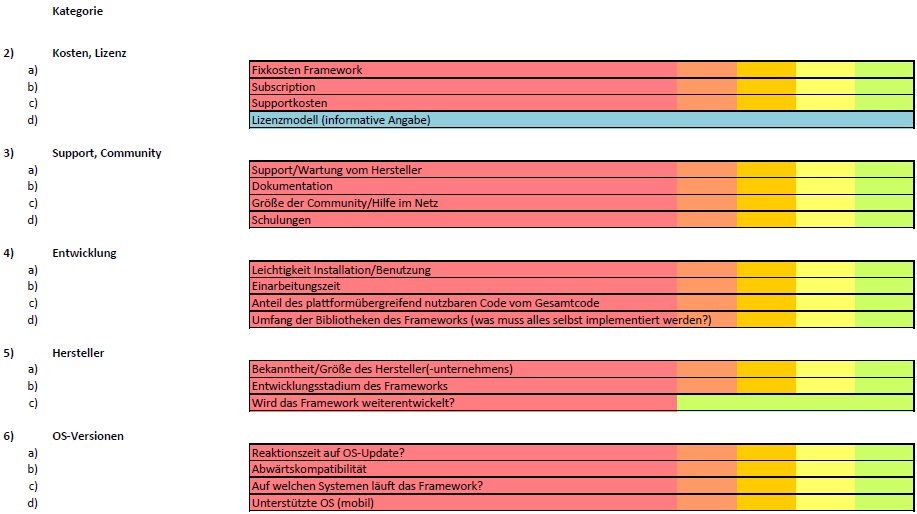
\includegraphics[width=1\textwidth]{Bilder/Bewertungsmatrix_1.PNG}
	\caption{Matrix der Bewertungskriterien, Teil 1}
	\label{fig:Bewertungskriterien_1}
\end{figure}

\section{Funktionsumfang}

In der Kategorie Funktionsumfang wird eine "Ja"-"Nein"-Unterscheidung bei der Fragestellung, welche Sensoren angesprochen und genutzt werden können, vorgenommen. Informationen darüber, welche Sensoren mit dem jeweiligen Framework genutzt werden können, bieten die jeweiligen Spezifikationen. Zusätzlich wird der Funktionsumfang der in Kapitel \ref{Marktanalyse} ausgewählten 3 Frameworks mit der Funktionstest-Anwendung praktisch getestet. So kann bei diesen Frameworks zusätzlich eine Bewertung über die Anwendbarkeit vergeben werden. Die Sensoren, die getestet werden sind: Der Beschleunigungssensor, der Lagesensor mit dem Gyroskop, das GPS, der Näherungs-sensor, das Magnetometer und das Barometer (siehe Abbildung \ref{fig:Bewertungskriterien_2}). 
\\
\\
Neben den oben beschriebenen Sensoren werden auch Funktionen wie die Benutzung der Front- und Rückkamera, der Zugriff auf das Dateisystem des Smartphones und Notifications getestet. Hier bekommen die in Kapitel \ref{Marktanalyse} ausgewählten Frameworks wie bei den Sensoren eine erweiterte Bewertung. Bei Punkt 6)6) "Kommunikation" fließt in die Bewertung mit ein, welche und wieviele unterschiedliche Kommunikationswege genutzt werden können, wie zum Beispiel Bluetooth oder WiFi. 

\section{GUI-Design}

Nur einen "Ja"-"Nein"-Unterschied gibt es bei den Punkten 7)1) "GUI-Designer" und 7)3) "integrierter Emulator", welcher schlicht besagt, ob diese Werkzeuge in dem jeweiligen Framework enthalten sind oder nicht (siehe Abbildung \ref{fig:Bewertungskriterien_2}). Punkt 7)2) Bei "Umfang der verfügbaren (nativen) UI-Elemente" wird getestet, welche unterschiedlichen Elemente des Android Material Designs einfach einsetzbar bar sind und für welche Elemente aufwändige oder weniger aufwändige Imports von Bibliotheken notwendig sind. Zudem wird der Aufwand bewertet entsprechende UI-Elemente in die Anwendung zu integrieren. 

\section{Interoperabilität und Erweiterbarkeit}

Punkte 8)1) "Webserviceaufrufe" und 8)2) "Bibliotheken von Fremdanbietern" werden mit einer "Ja"-"Nein"-Unterscheidung bewertet (siehe Abbildung \ref{fig:Bewertungskriterien_2}), d.h. es wird über-prüft, ob Webserviceaufrufe und Einbindung fremder Bibliotheken mit dem jeweiligen Framework möglich sind. Mit Punkt 8)4) "Support-Tools" wird bewertet, ob das Framework Support-Tools zur Verfügung stellt. Bei Punkt 8)3) "Integration in IDEs" wird ermittelt, wieviele unterscheidliche IDEs für die Entwicklung mit dem jeweiligen Framework einsetzbar sind, d.h. in wieviele IDEs das Framework integriert werden kann. 
\clearpage

\begin{figure}[h]
	\centering
	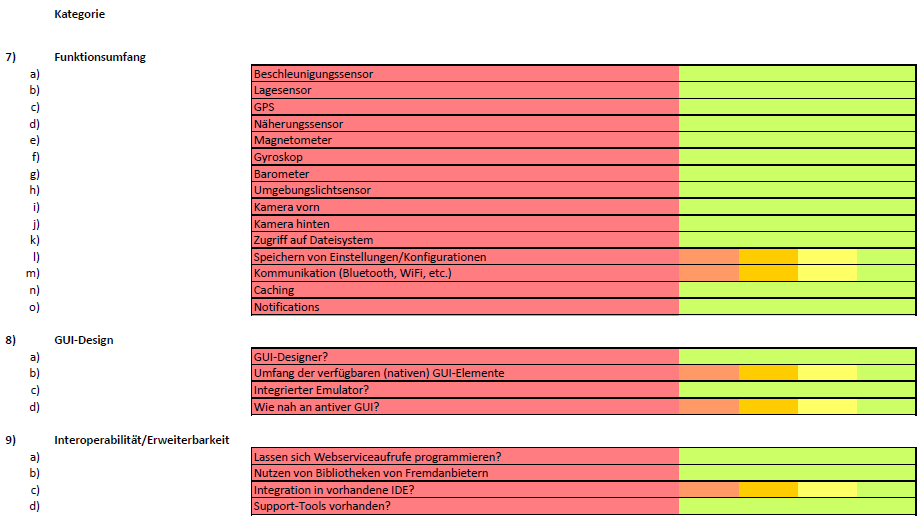
\includegraphics[width=1\textwidth]{Bilder/Bewertungsmatrix_2.PNG}
	\caption{Matrix der Bewertungskriterien, Teil 2}
	\label{fig:Bewertungskriterien_2}
\end{figure}

\section{Tests}

Bei den beiden Punkten 9)1) "Automatische Tests" und 9)2) "Test-Tools" (siehe Abbildung \ref{fig:Bewertungskriterien_3}) wird allein mit einer "Ja"-"Nein"-Unterscheidung bewertet, ob automatische Tests möglich und Test-Tools mit dem Framework ausgeliefert werden. 

\section{Performance}

Bei dem Bewertungskriterium "Performance" wird eine Abstufung entsprechend der Größe des Performance-Unterschieds zur nativen Anwendung vorgenommen. Auch wird die Größe der gebauten Installationspakete verglichen. 

\section{Sicherheit}

In dieser Kategorie werden folgende Fragestellungen beantwortet: 11)1): Wird das Rechtemanagement der jeweiligen Plattform nativ unterstützt? 11)3): Kann man Sicherheitszertifikate hinterlegen? 11)4): Kann ein eigener Zertifikatspeicher eingerichtet werden? 11)5): Werden VPN Verbindungen nativ umgesetzt (siehe Abbildung \ref{fig:Bewertungskriterien_3})? Zudem werden informative Angaben zu der Realisierung des Zugriffs auf Geräte-funktionen wie Speicher oder Kamera gemacht.  

\begin{figure}[h]
	\centering
	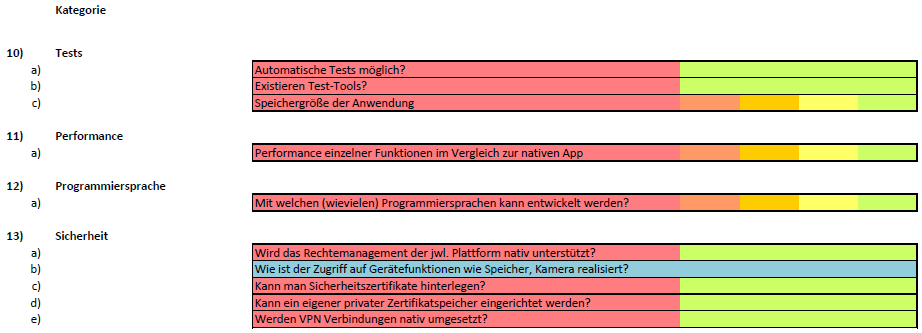
\includegraphics[width=1\textwidth]{Bilder/Bewertungsmatrix_3.PNG}
	\caption{Matrix der Bewertungskriterien, Teil 3}
	\label{fig:Bewertungskriterien_3}
\end{figure}